\documentclass[a4paper,twoside, openright,12pt]{report}
\usepackage{psfrag,amsbsy,graphics,float,amsmath,amssymb,epstopdf,xifthen,tikz,pgfplots,lscape,verbatim,bm}
\usepackage{graphicx, color} %deleted [dvips] in front of {graphicx, color} for usage with PDFLaTeX
\usepackage[latin1]{inputenc}
\usepackage[margin=15mm]{geometry}
\usepackage{verbatim} 
\pgfplotsset{compat=1.9}
\usepgfplotslibrary{groupplots}
\usetikzlibrary{matrix} 
%%% Stand 14.09.2007
%%% erstellt von Marion Sobotka
%%% marion.sobotka@tum.de
%%% last changes: 14.01.09


%_______Kopf- und Fußzeile_______________________________________________________
\usepackage{fancyhdr}
\pagestyle{fancy}
%um Kopf- und Fußzeile bei chapter-Seiten zu reaktivieren
\newcommand{\helv}{%
   \fontfamily{phv}\fontseries{a}\fontsize{9}{11}\selectfont}
\fancypagestyle{plain}{	
	\fancyfoot{}% keine Fußzeile
	\fancyhead[RE]{\helv\leftmark}% Rechts auf geraden Seiten=innen; in \leftmark stehen \chapters
	\fancyhead[LO]{\helv\rightmark}% Links auf ungeraden Seiten=außen;in \rightmark stehen \sections
	\fancyhead[RO,LE]{\thepage}}%Rechts auf ungeraden und links auf geraden Seiten
%Kopf- und Fußzeile für alle anderen Seiten
\fancyfoot{}
\fancyhead[RE]{\helv\leftmark}
\fancyhead[LO]{\helv\rightmark}%alt:\fancyhead[LO]{\itshape\rightmark}
\fancyhead[RO,LE]{\thepage}
%________________________________________________________________________________


%_Definieren der Ränder und Längen__________
\setlength{\textwidth}{15cm}
\setlength{\textheight}{22cm}
\setlength{\evensidemargin}{-2mm}
\setlength{\oddsidemargin}{11mm}
\setlength{\headwidth}{15cm}
\setlength{\topmargin}{10mm}
\setlength{\parindent}{0pt} % Kein Einrücken beim Absatz!!
%___________________________________________

%_Hyperref for CC Url__________
\usepackage{hyperref}
%___________________________________________

%_______Titelseite__________________________________________
\begin{document}
\pagestyle{empty}
\enlargethispage{4.5cm} %Damit das Titelbild weit genug unten ist!
\begin{center}
\phantom{u}
\vspace{0.5cm}
\Huge{\sc human behaviour modelling for teleoperation}\\
\vspace{1.5cm}
                                 \large{eingereichte\\
			  SEMINARARBEIT\\%/STUDIENARBEIT/MASTERRBEIT/BACHELORARBEIT\\ 
                                           von\\
                        %         \large{Zwischenbericht zur\\
			%DIPLOMARBEIT/STUDIENARBEIT/MASTERARBEIT/BACHELORARBEIT\\ 
			%		   von\\          

						\vspace{0.4cm}
					Martin Angerer\\
						\vspace{0.5cm}
					geb. am 10.06.1991\\
					wohnhaft in:\\
					Steinheilstr. 5\\
					80333 M\"unchen\\
					Tel.: 0151\,57978548\\
					\vspace{1.5cm}
					Lehrstuhl f\"ur\\
					INFORMATIONSTECHNISCHE REGELUNG \\
					Technische Universit\"at M\"unchen\\
					\vspace{0.6cm}
                    Univ.-Prof. Dr.-Ing. Sandra Hirche}
\end{center}
\vspace{5.0cm}
\begin{tabular}{ll}
Betreuer: Selma Musi\'c, M. Sc.  \\
Beginn: \hspace{10.5ex} 15.04.2016  \\
Abgabe: \hspace{9.8ex} 24.06.2016 \\
\end{tabular}
%____________________________________________________________

\newpage
\cleardoublepage



\phantom{u}
\phantom{1}\vspace{6cm}
\begin{center}
In your final hardback copy, replace this page with the signed exercise sheet.
\end{center}

\newpage


%_______Abstract_____________________________________________
\topmargin5mm
\textheight220mm
\pagenumbering{arabic}
\phantom{u}
\begin{abstract}
The human behaviour is very complex and cannot be captured with a single model. Dependent on the role of the operator in a teleoperation task, various models are known in literature. The range of applications and modelling approaches is diversified. According to Sheridian \cite{Sheridian1992} the human behaviour is determined by three major aspects: Sensory perception, cognition and response.
Response or motor function modelling is mostly concerned with what the human \emph{can} do based on the limitations imposed by the human physiology. Cognitive models focus on what the human \emph{will} do in a certain situation. Sensory perception modelling helps to determine which information is useful, and which cannot be perceived by human. All three aspects are beneficial for control design. This paper provides an overview on existing human modelling approaches in literature. A special focus is put on which methods are applied in direct, shared and supervisory control.
\begin{center}	
\normalsize \textbf{Zusammenfassung}\\
\end{center}
Hier die deutschsprachige Zusammenfassung
\end{abstract}
%____________________________________________________________

\newpage

%_______Widmung_______________________________________________
\phantom{u}
\phantom{1}\vspace{6cm}
\begin{center}
%Hier die Widmung oder leer lassen
\end{center}
%_____________________________________________________________



\pagestyle{fancy}

%_________Inhaltsverzeichnis__________________________
\tableofcontents 
%_____________________________________________________



%_________Einleitung__________________________________
\chapter{Introduction}

Teleroperation is a general term for remote control of physical systems by humans through the mediation of computers. Despite large efforts towards autonomous systems, human operators are indispensable in many non-repetitive or unpredictable tasks. Human perception, planning and control are still required in unstructured environments that are not accessible or hazardous for human workers, such as outer space, deep water, nuclear contaminated areas, or a battlefield.\\
Remote control in order to replace a human in dangerous situations often uses master-slave mechanical manipulation. The operator directly controls the remote robot, which has little or no autonomy. Today's robots possess mature sensory functions and high level planning capabilities that allow them to operate independently of human control most of time. Nonetheless a human is still necessary for monitoring, detection of abnormalities and intervention when necessary \cite{Sheridian1992}.\\
Independent of the level of autonomy of the robotic system it is the objective of control design to maximize the benefits of human-robot cooperation. The modelling of human sensing, cognition and actuation opens insights how to provide information to the user, support decision making and design the user interface. This term paper reviews approaches which exploit human modelling in teleoperation to enhance the joint performance of humans and robots.
Dependent on the role of the human in the control loop, different aspects of human modelling apply. Roughly the following architectures are distinguished for a human in the loop.

\subsubsection{Direct, shared and supervisory control} 
In direct control approaches humans operate the robot without any automated help, e.g. by manipulating a haptic device. On the other hand, applying supervisory control, the robotic teams act autonomously and the operator issues high-level commands, e.g. "relocate to a certain place" or "grasp an object" \cite{Peters2015}. The operator continuously receives information on the state of the robotic system and periodically issues commands, thus rather oversees and directs than controls the system \cite{Sheridian1992}.
The intermediate between supervised and directly controlled systems are shared control systems. At least some local, low-level feedback loops refine the robot behaviour to assist the operator in high-level task execution \cite{TeleoperationHandbook}.\\
The performance in directly controlled manipulation is largely influenced by the motoric functions of the operator, while in supervisory control the human decision making comes to fore. This motivates a coarse differentiation of human modelling sub-domains. 

\subsubsection{Sensory perception, Cognition and Response (SCR)}
The SCR paradigm is a general classification of the behavioural activity of a human. The modelling of human perception encompasses one or several sensory organs (vision, touch, hearing,...). Cognitive activity refers mainly to decision making, planning and learning. Response or motor functions describes the skeletal-muscular potential and is thus the physiological component of human modelling. Clearly, there are overlaps between the classes, e.g. humans are susceptible to information overload, perception depends also on the mental state of the operator. Nevertheless his paper is structured based on the SCR-classes, we will see that sophisticated approaches span more than class of human modelling.\\
The remainder of the paper is organized as follows: \textbf{Chapter 2} divides into the 3 classes of SCR.\\
\textbf{Section 2.1} is dedicated to to response or motor function modelling. The review starts with the class, which has the clearest impact on performance and stability in teleoperation.\\
\textbf{Section 2.2} has the sensory perception modelling ...\\
\textbf{Section 2.3} introduces the broad field of cognitive modelling in teleoperation. Starting from decision making between two choices, the upper bound of human cognition modelling is reached with the general purpose mental model \emph{ACT-R}.\\
\textbf{Chapter 3} draws a brief conclusion.
  




\section{Problem Statement}






%____________________________________________________



%_____Kapitel 2_________________________________
\chapter{Main Part}
\section{Response or motor function modelling}
\subsubsection{Bilateral telemanipulation}\label{SS:BilateralTelemanipulation}
Motor function modelling is mainly motivated by master-slave manipulation. The human manipulates a \emph{teleoperator} (the master robot) and the \emph{teleroobot} (slave) follows the masters motion \cite{TeleoperationHandbook}. In return the human is provided with force-feedback of the resistance found by the telerobot. Thus, by manipulating the teleoperator, the human enforces a relation between force and velocity. At the level of interaction the human is a mechanical impedance. In a seminal work Hogan \cite{Hogan1989} investigates the dynamics of a human arm. Although the human arm is actively controlled by neuro-muscular feedback, it is indistinguishable from a passive impedance. To ensure closed-loop stability it is common to render each subsystem of a teleoperation set-up passive \cite{Niemeyer2004}. An overview of a common teleoperation set-up is shown in figure \ref{FIG:TeleoperationScheme}. This generates a high stability margin and results in conservative control design. If the communication line exhibits delays, its passivation leads to a distorted display of the manipulated environment to the human. To achieve stability it is sufficient if the closed loop in sum dissipates energy. Instead of passivating every element, the energy balance of the closed loop is analyzed in terms of \emph{dissipativity-based control}. Dissipativity is a generalization of passivity with respect to a more general definition of energy transfer. A system is called dissipative if there exists a positive semi-definite energy function $V$ such that
\begin{equation}
\dot{V}(x(t)) \leq s(u(t),y(t)),
\end{equation}
where $x$ is the state, $u$ the input and $y$ the output of the system. The supply rate is $s(u(t),y(t)) = y^T(t)u(t)$ for the special case of a passive system.\\
The interconnection of multiple dissipative systems $\Sigma_i, \, i=1...N$ with supply rates $s_i(t)$ is again a dissipative system $\Sigma$ with the summed supply rate $s(t)=\sum_{i=1}^N s_i(t)$ .
The combined system $\Sigma$ is locally stable (in the sense of Lyapunov) if $s(t)$ is locally negative semi-definite. Clearly this means that more energy is withdrawn then supplied to the system \cite{Varnell2013}. Some components may be active with a positive supply rate, if other components dissipate more energy at the same time.\\
One system component that is guaranteed to be dissipative at all times, is the human operator manipulating the haptic device (teleoperator). Identification studies \cite{Rahman1999} of the human arm show that it is inherently damped. A minimum damping $d_{\text{h,min}}$ is identified, which is the guaranteed dissipation.\\
The passivation of the communication channel e.g. using the wave/scattering transformation \cite{Niemeyer2004}, results in a distorted display of the environment. If this component is designed active, exploiting the guaranteed dissipation of the other systems portions to maintain stability, the displayed environment will be more realistic. A more realistic perception of the task can improve the human performance in teleoperation. The \emph{generalized wave/scattering transformation} \cite{Hirche2012} uses the guaranteed dissipation of the other components to design an active communication channel. Thereby the closed loop system is still dissipative. This is done by specific choices of the transformation matrices. The reproduction of this procedure is beyond the scope of this paper, please refer to \cite{Hirche2012} directly.
\begin{figure}
	\centering
	\footnotesize
	\def\svgwidth{1\columnwidth}
	\input{TeleoperationScheme.eps_tex}
	\caption{Structure of a general teleoperation system}
	\label{FIG:TeleoperationScheme}
\end{figure}

\subsubsection{Pointing interfaces}
The haptic interfaces considered in the previous subsection are often tailored to a specific problem and/or a specific robot. Pointing interfaces like a computer mouse or a touch-screen tablet are versatile and cost-efficient. However, different modelling approaches for the human dynamics have to be considered. When manipulating a pointing device (mouse, touch-screen) the human does not receive force feedback, thus the impedance models do not apply. The human pointing dynamics are studied both theoretically and experimentally (system identification).\\
The \emph{vector integration to endpoint} (VITE) model is a neural command circuit to generate human arm trajectories \cite{Varnell2013}. In the simplest form it is written as 
\begin{align}
\dot{\nu} &= \gamma(-\nu + x_d - x) \\
\dot{x} &= G(t) \max(0,\nu), \nonumber
\end{align}
where $\nu$ expresses the deviation between the target arm position $x_d$ and the actual arm position $x$. $\gamma$ is a positive constant. The \emph{GO} signal $G(t)\geq 0$ indicates the human to correct the deviation. The human arm manipulates the pointing device, thus the dynamics of the human arm describe the pointing dynamics. The pointing behaviour is dissipative as long as $\nu \geq 0$ \cite{Varnell2013}. The case of $\nu < 0$ clearly represents a position overshoot ($x>x_d$). Fast human motions typically result in an overshoot. Clearly there is a tradeoff between an overshoot and the time to reach the target.\\
If the target position is known to the input interface, e.g. in a trajectory following task, the interface can remove the overshoot from the human input. The resultant pointing dynamics is then guaranteed dissipative. If the human performs arbitrary tasks, the motion target is not known to the interface. Consequently the human may be active at some point. Other components of the teleoperation system then have to be dissipative to form a dissipative closed-loop system (see also \ref{SS:BilateralTelemanipulation} for interconnected dissipative systems). In \cite{Varnell2013} the analysis of the pointing dynamics serves to ensure stability for the direct teleoperation of a single robot.\\
On the experimental side, recent work \cite{Hatanaka2015} performs system identification of the pointing dynamics in the frequency domain. The user study indicates that humans performing pointing tasks are passive at low frequencies($f\leq 1 \text{[rad/s})$. The augmentation of the higher frequency components by a high-pass filter makes the human decrease the gain for these frequencies. In addition the high-pass filter introduces an additional stability margin into the loop. System identification of the filtered system then indicates passivity below frequencies of $10 \text{[rad/s}$. Thus the human pointing dynamics are found to be passive at the frequencies of interest. In \cite{Hatanaka2015} this knowledge serves to show that a swarm of robots asymptotically achieves synchronization, even if a human controls only a part of the swarm.\\







\subsubsection{Mobile human sensors and actuators}
Unautomated, extensively distributed control systems require the operator to travel between the locations where control actions are performed. One typical example are irrigation canals in low-tech countries. The canal managers shuttle between the gates, take measurements and adjust the actuators based on their local knowledge and their experience of the overall system behaviour. Despite being complex dynamical systems, irrigation canals are mathematically tractable and for some canals detailed models already exist \cite{vanOverloop2015}. Modelling allows the prediction of the canal's state from a known initial condition. \emph{Model-predictive control} (MPC) computes the current control action in order to reach a future optimal system condition. Common MPC schemes operate automatically based on continuous sensor readings and automated actuators.\\
MPC can serve as a high-level control for an irrigation canal operated manually by humans. In contrast to fully automated MPC schemes, sensory information is only available from the current location of the operator. Similarly control actions can only be performed on the spot. Whenever the operator travels between the gates, no measurements or control actions are possible. If the high-level MPC requests a certain measurement or actuation, then this usually results in a significant delay, because the operator has to relocate to the spot. Therefore the human dynamics (i.e. travelling speed) have to be considered in the system model. \\
The role of the human in the control loop is reduced to be a mobile sensor and actuator. The high-level planning and control is accomplished by automatic MPC. One can say that not a human teleoperates the system, but the human \emph{gets teleoperated}. The modelling of the human reduces to describe the speed of task execution. The elapsed time, until a requested measurement bescomes available or a control action is performed, is a delay. Thus the human dynamics is suitable represented by delays. Instead of speaking of a human-in-the-loop system, the problem can also be viewed as a distributed control system with partially delayed communication.\\
The model of the canal system is divided into $i=1...N$ discrete pools, which are separated by gates. The simulation is time-discrete with sampling time $T_s$. The system description starts from a linear model of the $i$-th canal pool
\begin{equation}
x_i(k+1) = x_i(k) + \frac{T_s}{c_i}(q_{i-1}(i) - q_i(k) + u_i(k)).
\end{equation}
The state $x_i(k)$ represents the water level at time step $k$. The inflow from the upstream pool $i-1$ is denoted by $q_{i-1}$. The downstream outflow is $q_i$ and the flow to/from external sinks/sources is given by $u_i$. The flows $q_{i-1},q_i$ can be controlled manually by the setting the respective gate positions. The surface area of the pool is denoted with $c_i$.\\
The desired water levels $x_{\mathrm{ref},i}$ are known in advance and constant. The objective of MPC is to reach an optimal system state by anticipatory control. Here the optimality condition is to minimize the deviations of actual and desired water levels while keeping the number of control actions small. This results in a minimization problem over a finite prediction horizon $N_p$ \begin{align}\label{EQ:MoMPCcostfunction}
\min_{\Delta q_i (k:k+N_c)} \sum_{l=0}^{N_p-1} \sum_{i=1}^{N} &\Delta x_i^T(k+l) Q_i \Delta x_i(k+l) + Q_{\mathrm{l},i}^T \Delta x_i(k+l) \\  &+ \Delta q_i^T(k+l) R_i \Delta q_i(k+l) \nonumber,
\end{align}
where $\Delta q_i = q_i(l+1) - q_i(l)$ is the change of flow during one timestep. The deviation of the water level is $\Delta x_i (l) = x_i(l) - x_{\mathrm{ref},i}$. The matrices $Q_i,Q_{\mathrm{l},i},R_i$ are constant weighting matrices. The linear term associated with $Q_{\mathrm{l},i}$ accounts in this context for pumping costs.\\
 The result of solving the optimization problem (\ref{EQ:MoMPCcostfunction}) is the change of a flow $\Delta q_i$ at gate $i$. A change of flow is realized by the operator manipulating the gate setting.  Recall that control actions are only feasible if the human is on the spot. This is taken into account by imposing constraints on the minimization task, namely $\Delta q_i(k) = 0$ whenever the operator is not at location $i$ at the time $k$.\\ 
The MPC computes a sequence of control actions from timestep $k$ to $k+N_c$. The sequence over the control horizon $N_c$ instructs the operator which measurement or control action is the next to accomplish. Thus the MPC also achieves an optimal task scheduling for the operator.\\
For simplicity only a single operator is considered so far. In \cite{vanOverloop2015} multiple operators travel between the gates. Modelling and optimization formulations are equivalent to the ones shown. For the constraints on the optimization task, one requires that $\Delta q_i(k)=0$, whenever \emph{no} operator is at gate $i$. 


%Hirche and Buss exploit the guaranteed damping to design a closed loop that is dissipative although not all sub-parts are passive. In sum the connected elements are still dissipative, but the communication system is designed less conservative. Thereby the displayed environment gets less distorted.  
%The interconnection of \emph{per se} passive sub-systems results in an overly conservative teleoperation system. If the communication line exhibits delays, its passivation leads to a distorted display of the manipulated environment to the human. Hard objects are displayed softer and the transmitted inertia in free-space motion is increased. Overly conservative control design affects the operator-perceived environment and hinders the operator's performance.\\
%The human arm impedance is highly adaptive, the principle of antagonist muscles enables the human to willingly change the stiffness by activating both muscles \cite{Rahman99}. With the stiffness also the damping of the arm changes, if a minimum damping is guaranteed , the control design can be less conservative. Rahman et al. determined a minimum damping using system identification, this guaranteed dissipation is exploited to design a dissipative closed loop system, while the not all components must be passive. 
%By using more knowledge of the human physiological dynamics, the distortion of the displayed environment is reduced.\\
     
\section{Sensory perception modelling}
Human performance in teleopeation is highly dependent on how the human perceives the remote environment. In fine manipulation tasks and for correct decision making it is essential that the operator receives accurate feedback. Typically visual and haptic feedback is provided, while occasionally other senses like hearing are addressed. In the ideal case the human can not distinguish the virtual from the remote environment, then the teleoperation system is \emph{transparent} \cite{Hirche2012}.\\
The stabilization of a teleoperation system in presence of communication delays distorts the haptic display of the environment (see the subsection \ref{SS:BilateralTelemanipulation}). Hard objects are displayed softer and the free-moving telerobot is displayed with an increased inertia. Transparency is thus not achievable. The human perception resolution is limited, e.g. we cannot distinguish different weights that are within a certain range. To a certain extent a hard object can be displayed softer, or a body can be displayed more inert and the human does not notice the difference. The concept of taking advantage of the sensory inaccuracy of the human is called \emph{perceived transparency}.
For example, a typical human cannot sense a difference inertias within a range of 21\% difference, the just noticeable difference (JND) in stiffness is around 8\% \cite{Hirche2012}.\\
The passivation of the communcation channel with the popular generalized wave/scattering transformation \cite{Niemeyer2004} can be tuned to transmit either stiffness or inertias  approximately correct. Good transparency in free-space motion and for stiff contacts is not achievable at the same time. The impedance $Z_h$ displayed to the human, transmitted over a passivated, delayed communication channel, is related to the original impedance $Z_e$ by
\begin{equation}
Z_h (s) = b \frac{1+R(s)e^{-sT}}{1-R(s) e^{-sT}} \text{  with  } R(s) = \frac{Z_e(s) - b}{Z_e(s)+b}.
\end{equation}
The formulation is given in the Laplace domain with $s$ being the complex frequency parameter. The delay of the communication channel is denoted with $T$. The wave impedance $b$ is the tuning parameter. In the following, it becomes apparent how the tuning gives conflictive results for the accurate display of inertias and stiffness. In free-space motion the environment exerts no force on the telerobot, i.e. the environment impedance is $Z_e=0$.  After a number of simplifications (see \cite{Hirche2012}), the low-frequency approximation of the impedance displayed to human is
\begin{equation}
Z_h^*(s) = \frac{bT}{2}s
\end{equation}
A small wave impedance $b$ leads to a small distortion of the displayed impedance, in particular $\lim_{b\rightarrow0} Z_h^* = Z_e$.\\ 
A stiff environment is described by the transfer function $Z_e = k_e/s$, with a stiffness parameter $k_e$. The low-frequency approximation of the displayed impedance is
\begin{equation}
Z_h^*(s) = \frac{2k_e b}{2b+k_e T}\frac{1}{s}
\end{equation}
In this case a high wave impedance $b$ leads to a correct display of the environment, $\lim_{b \rightarrow \infty} Z_h^* = Z_e$. Thus there is a conflict of objectives when tuning $b$. \\
To illustrate how the perception resolution is used for control design, consider a fine manipulation task. To achieve the best performance it is important to display the exact stiffness of the environment to the operator. The free-motion dynamic is subordinate. The wave impedance is now chosen to keep the stiffness distortion due to the wave transformation just not noticeable for the human
\begin{equation}
b > (1-\mathrm{JNR}_k) \frac{k_e T}{2}, 
\end{equation}
where $\mathrm{JNR}_k$ is the just not noticeable threshold for stiffness. Conclusively, by considering the human perception resolution the displayed free-motion dynamic becomes more realistic without compromising the perceived stiffness.  
     
\section{Cognitive modelling}
Cognitive modelling seeks to give a reliable prediction of the human behaviour in certain situations. The complexity of the models depends highly on the desired prediction horizon and the and the amount and structure of the available information.\\
The simplest, conceivable model of human behaviour is to assume that the human behaviour will not change over the prediction horizon. The so-called \emph{zero order hold} extrapolation is successfully used in model-predictive control of a quadruped robot \cite{Chipalkatty2013}. In a shared control approach, the human controls the front legs, while the rear legs are automatically placed to ensure gait stability. Furthermore human inputs are subject to stability constraints, i.e. with a given rear leg position only certain movements are allowed. Human behaviour prediction helps to position the rear legs in a way that allows to preserve the human intent. The prediction horizon in this problem is fairly short. In fact zero-order hold extrapolation is preferred over more complex methods. First-order hold or least-squares system identification reflect longer term trends in the user inputs \cite{Chipalkatty2013}. In a user study the simple zero-order hold method is found to be the most helpful prediction method. The participants are faster in task-completion and experience less workload compared to the more complex methods. \\
\subsubsection{Learning}
Teleoperation is commonly used for complex tasks in unstructured environments humans cannot easily access, e.g. space construction. For most tasks a direct human control is preferred but there are some repetitive tasks the robot can perform autonomously. Examples are grasping a standard object or tightening a screw. Such fine manipulation tasks are challenging for a human, if the feedback is distorted due to communication delays (see \ref{SS:BilateralTelemanipulation}). Moreover the human behaviour is inherently stochastic, i.e. even an experienced operator shows occasionally poor performance. Poor performance in space construction is undesired because it may result in an irretrievable loss of parts or tools. One particular solution proposed in \cite{Yang1994} is to \emph{teach} the telerobot a set of motion patterns while it is still on earth. The motion sequences are captured from a human operating the robot   via teleoperation, just as in the space application. The important difference is that there is no delayed communication, i.e. the operator receives undistorted feedback. And second, only good sequences can be selected from a number of total attempts.\\
In the space application a human controls the trained robot by teleoperation. The robot observes the human commands and if it recognizes one of the learned sequences with sufficient probability, it switches to automatic control. The operator continues to carry out the task. The robot only performs the recognized task automatically if there is a sufficient accord with the human input. At the moment the human deviates significantly from the recognized trajectory, the robot executes the human command. Ideally the human can not distinguish between automatic and teleoperated task execution. The automatic mode performs the same task but does suffer from minor inaccuracies, because it repeats a "good" sequence. By default the human is in control, only for some reptetive tasks the automatic controller takes other control. Therefore the approach is classified as \emph{traded control} \cite{Sheridian1992}.\\
Technically  the basis of Yang's \cite{Yang1994} approach is \emph{learning from demonstration}. One of the major difficulties when transferring human skill to a robot is the randomness of human actions. Human motion is even doubly stochastic. The intention what the human deserves to do is dependent on many factors and must be considered a random variable. Furthermore it is not directly measurable or observable. Second, the physical movement of a human is also stochastic, two motion sequences carried out after each other are never exactly identical. Since the intention of the human is hidden to the learning robot, is must be estimated based on the observed motion. This motivates the use of \emph{Hidden Markov Models} (HMM), with the intention being a state $X_i$ in the \emph{Markov} chain and the motion sequence being the observation $Y_k$ \cite{Yang1994}. The transition from state $i$  to state $j$ is assigned with a transition probability $a_{ij}$. The possibility to be in a state $i$ and make the observation $k$ is described by $b_{ki}$. Figure \ref{FIG:HiddenMarkov} illustrates the relations for an object grasping task.
\begin{figure}
	\centering
	\footnotesize
	\def\svgwidth{1\columnwidth}
	\input{HiddenMarkov.eps_tex}
	\caption{Hidden Markov model (left) with measured motion sequence and estimated states $\tilde{X}_i$}
	\label{FIG:HiddenMarkov}
\end{figure} 
Collecting all transition probabilities entails in a transition matrix $A \in \mathbb{R}^{N \times N}$ (for $N$ total states), the observation probabilities are concentrated in the matrix $B \in \mathbb{R}^{N \times M}$. A HMM $\lambda = (A,B,\pi)$ is fully described by a transition matrix, a observation matrix and the initial state distribution $\pi$. Learning means to adjust the parameters of the HMM to maximize the probability $P(O \mid \lambda)$ that the model matches the observation sequence $O=(Y_1...Y_M)$. The parameter optimization process is commonly done with the backward-forward algorithm, for details refer to \cite{Yang1994}. For one task (e.g. grasping an object) multiple motion sequences $(O_1...O_R)$ are used for training, each of them results in different optimal parameters. Thus for $R$ training sequences one obtains $\lambda_r \, r=1...R$ different HMMs. In the space application the telerobot receives the input sequence $O^*$. The objective is to select the best fitting trajectory from all learned ones. This can be done using the \emph{Bayes} formula
\begin{equation}
\max P(\lambda_r \mid O^*) = \frac{P(O^* \mid \lambda_r) P(\lambda_r)}{P(O*)} \; , \; \forall r=1...R
\end{equation}
If the maximum probability is above a certain threshold the controller executes the learned trajectory. For every new observation the telerobot receives from the operator the probabilities are updated. Thus with every new input another learned trajectory can be pursued or, if no HMM reaches the required probability $P(\lambda_r \mid O^*)$, the human input is executed directly.
%
%Often no clear criteria what is good performance in complex tasks exist. Based on the assumption that an experienced human shows usually good performance, the learning goal is to make the HMM reproduce the most likely human performance.\\
%Learning certain motion patterns from an experienced user allows the robot to perform the learned task automatically. The role of the human in teleoperation is reduced to supervision \cite{Yang1994}. 

\subsubsection{Decision making}
In general human decision making is influenced by previous experience and by the actual sensory perception. Knowledge and experience differ highly between various subjects and are difficult to model, therefore models on decision making focus on measurable inputs (perception).\\
The aim of decision making modelling in teleoperation is not to replace the human but to provide support. Automatic suggestions guide the workflow and have to approved or rejected by the human as a final instance. Another possibility is to withdraw some low-level decision making tasks from the user's responsibility, to allow focus on the superordinate strategy.\\
The simplest decision tasks are two alternative choices, complexity increases significantly with multiple alternatives. Most studied and best characterized are two alternative choice tasks. Over time the human perceives information that is classified in favour of one of the two alternatives. A decision is either taken if a threshold of certainty for one alternative is reached, or by choosing the more probable alternative after a fixed evaluation time. The \emph{Drift Diffusion Model} (DDM) is frequently used to model human decision making based on sensory perception. The DDM describes the cognitive process that leads to choices between two alternatives. Decisions are taken in a noisy process, which starts from a neutral or biased point and evolves by the accumulation of information. The rate of accumulation of information is called the drift rate $\mu$. The rate increases with the quality of perceived information. Quality here means how good the information matches one alternative. Human sensory perception is noisy. The decision making process contains a stochastic element, described with standard \emph{Wiener process}.    The evidence accumulation of the DDM is characterized by a stochastic differential equation 
\begin{equation}
dx(t) = \mu dt + \sigma dW(t),
\end{equation}  
where $\sigma$ is the diffusion rate. It characterizes the influence of the stochastic noise on the accumulated evidence $x(t)$.\\

\begin{figure}
\centering
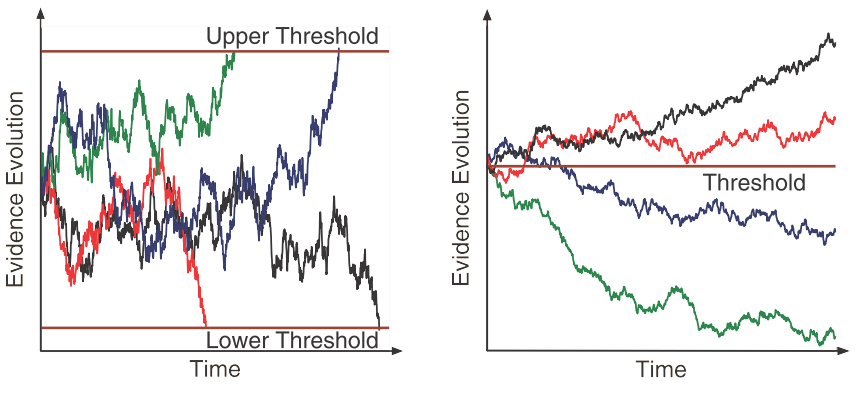
\includegraphics[width=1\linewidth]{EvidenceAcc.png}
\caption[Decision making by evidence accumulation]{Decision making by evidence accumulation: decision thresholds (left) and fixed evaluation time \cite{Peters2015}}
\label{FIG:EvidenceAcc}
\end{figure}

The choice of the thresholds that lead to a decision, or the pre-defined evaluation time, represent a trade-off between speed and accuracy. Several methods for an optimal choice in terms of maximizing efficiency or minimizing risk are formalized in literature \cite{Peters2015}.
Multiple alternative choices with disjoint objectives can be evaluated with separate accumulation processes in a \emph{race model}. There is an individual stochastic process for each alternative $i=1...N$
\begin{equation}
dx_i(t) = \mu_i dt + \sigma dW_i(t)
\end{equation}
 A decision is either taken if one alternative reaches a defined evidence threshold, or after the fixed evaluation time has elapsed the most evident alternative is chosen. Figure \ref{FIG:EvidenceAcc} illustrates the processes.\\ Having to choose between multiple options is much more difficult for a human than to choose from two options. As a consequence the reaction time increases. For the modelling of multiple-choice decision making with race models, \emph{Hick's law} is an estimation for the increase of reaction time. For $N$ alternative choices, the reaction time increases at a rate proportional to $log(N)$.\\
For a task with many periodic and well structured decisions, a model of the human decision making can support the human by reducing the workload.  For example in the persistent surveillance mission described in \cite{Peters2015} the operator monitors the sensor data of multiple autonomous agents. A decision support systems pre-selects critical incidents the operator should focus the attention on. The sensor data is automatically searched for abnormality indcations, a model of human decision making determines wheter the case is presented to the operator. By forecasting the evaluation time it takes the human to analyse the scene, the tasks are efficiently scheduled and a maximum number of critical cases can be processed in the given time \cite{Bertuccelli2010}. This a allows a human to supervise a larger number of autonomous agents than without a decision support system.\\
The cases to be decided by the human are queued. A minimum stability requirement is imposed on the queue length. Furthermore the queue should always be short to allow for a close to realtime processing of an incident. With the number of agents supervised by an operator the rate of cases,  which can be decided by the operator, decreases. Therefore suitable modelling of the decision making      reduces human-resource allocation.
        






%_______________________________________________



%_____Zusammenfassung, Ausblick_________________________________
\chapter{Conclusion}
From a control point of view the human is a complex dynamical system. Clearly no single model is capable of capturing all the aspects of human behaviour. The existing modelling approaches for teleoperation are diverse and tailored to the application. This paper highlights several solutions in consideration whether they apply for direct, shared or supervisory control.\\
Probably the most researched human models apply for bilateral telemanipulation. The inherent dissipation of human motion can be exploited to enhance the transparency of the teleoperation system. Bilateral telemanipulation also benefits from the modelling of the human perception resolution. Just not noticeable differences in haptic perception serve as a guideline for parameter tuning in communication channel passivation. Bilateral telemanipualtion requires a haptic interface, in contrast to that simple pointing interfaces (mouse, touch-screen) become increasingly popular. The resulting motion dynamics is covered both by theoretic modelling and by experimental system identification. Namely the VITE model for pointing behaviour is largely unexplored in literature and may be an interesting field of future research.\\
Human cognition processes are even more difficult to model than motion and perception. Nevertheless even simplistic models are beneficial for system performance. Assuming the operator to pursue the current action is often correct for a small prediction horizon. A human and model-predictive controller share control of a quadruped robot. By predicting no change of the human input, the controller places the rear legs to maximize the freedom of the teleoperated front legs. A space construction application shows how human motion sequences can be stored in Hidden Markov Models. Trading the control automatic execution of the learned patterns can eliminate minor uncertainties in repetitive tasks.
Automated image analysis can serve as a decision support system in the supervision of multiple UAVs. Therefore the human decision making is modelled to pre-select the vast amount of images and display only the interesting ones to the human.\\      
Human modelling can improve the  interaction of humans and robots in various ways. With the exception of the bilateral telemanipulation, for all other problems the modelling of the human for teleoperation is only at the beginning.  



%_______________________________________________________________


%_____Abbildungsverzeichnis_________________________________
\cleardoublepage
\addcontentsline{toc}{chapter}{List of Figures} 
\listoffigures 	 %Abbildungsverzeichnis

%___________________________________________________________

%_____Literaturverzeichnis_________________________________
\cleardoublepage
\addcontentsline{toc}{chapter}{Bibliography}
\bibliography{MyCollection}
\bibliographystyle{alphaurl}
%__________________________________________________________


%_____License_________________________________
\cleardoublepage
\chapter*{License}
\markright{LICENSE}
This work is licensed under the Creative Commons Attribution 3.0 Germany
License. To view a copy of this license,
visit \href{http://creativecommons.org/licenses/by/3.0/de/}{http://creativecommons.org} or send a letter
to Creative Commons, 171 Second Street, Suite 300, San
Francisco, California 94105, USA.
%__________________________________________________________

\end{document}
